\capitulo{3}{Conceptos teóricos}

En este apartado se desarrollan los conceptos necesarios para comprender el funcionamiento de la aplicación que se ha desarrollado en el presente trabajo.

\section{Visión artificial}

La visión artificial, también conocida como visión por computador, es un subcampo de la inteligencia artificial que trata los métodos para adquirir, procesar, analizar y comprender imágenes y,
en general, datos de varias dimensiones obtenidos del mundo real con el fin de obtener información
numérica o simbólica\cite{wiki:artificial}.
Se puede describir también como el proceso de extracción de información del mundo físico a partir de imágenes utilizando para ello un computador 

\section{OCR} \label{ocr}

OCR(Optical character recognition) es la conversión mecánica o electrónica de imágenes, que contienen texto, ya sea escrito a mano, o impreso por una máquina  a texto editable.
Esta técnica es ampliamente utilizada para digitalizar textos impresos, para poder ser utilizados en otros procesos, como por ejemplo síntesis de texto a voz, o traducción de documentos. \cite{ocr}

A continuación se describen los pasos para esta transformación.

\subsection{Pre-Procesado}
En esta etapa, las imágenes son tratadas para mejorar la exactitud a la hora de su transformación.

\begin{enumerate}
	\item \textbf{Inclinacion:} \label{deskewing} A la hora de escanear documentos, estos pueden no estar alineados correctamente, por ello es necesario girarlas unos grados, para poder colocar las lineas de texto en vertical u horizontal.Para ello se emplea un algoritmo de “deskewing”.
	Este proceso permite enderezar la imagen a partir de un angulo , el cual es posible calcular, por ejemplo con la Transformada de Hough(ver sección\ref{Hough}).
	\imagen{desviacion_1}{Desviación del texto, y su tangente para alineación}
	
	\begin{figure}[ht]
		\centering
		\begin{minipage}[b]{0.45\linewidth}
			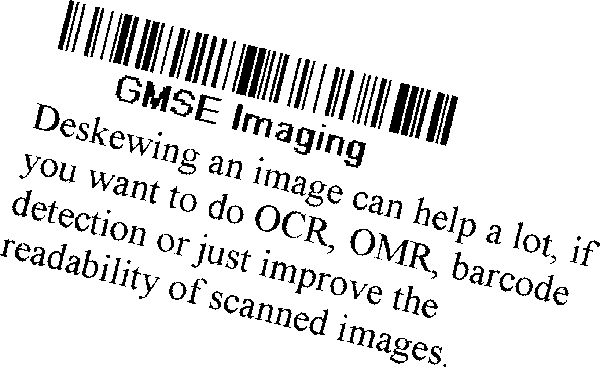
\includegraphics[width=\linewidth]{inclinacion1.png}
			\caption{Imagen antes de aplicar un algoritmo de deskewing }
			\label{fig:minipage1}
	\end{minipage}
	\quad
	\begin{minipage}[b]{0.45\linewidth}
		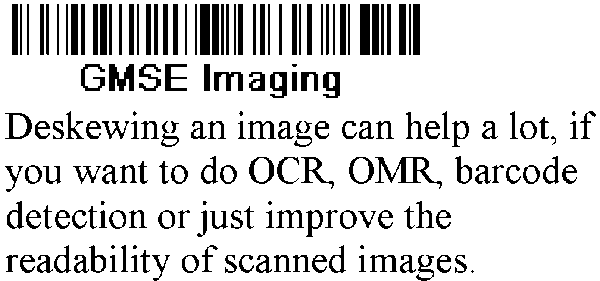
\includegraphics[width=\linewidth]{inclinacion2.png}
		\caption{Imagen después de aplicar un algoritmo de deskewing}
		\label{fig:minipage2}
		\end{minipage}
	\end{figure}

	\item \textbf{Binarización:} Transformar una imagen en color, o en escala de grises a blanco y negro, por ello se la denomina imagen binaria.
	
	\item \textbf{Eliminación de lineas:} Consiste en la eliminación de lineas de texto y cajas en las que el texto pueda estar incrustado (ver figura \ref{fig:lineas}).
	\begin{figure}[ht]
		\centering
		\begin{minipage}[b]{0.45\linewidth}
			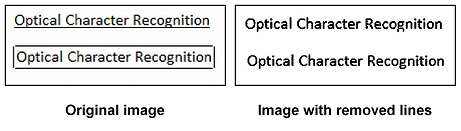
\includegraphics[width=\linewidth]{lineas1.png}
			\caption{Eliminación de lineas en un OCR}
			\label{fig:lineas}
	\end{minipage}
	\end{figure}
	\item \textbf{Zoning:} En esta etapa, el OCR detecta las posiciones de los elementos importantes de la imagen, por ejemplo columnas, párrafos etc..
	\item \textbf{Detección de lineas y palabras:} Se encarga de encontrar las lineas de texto y separarlas por palabras si es necesario.
	\item \textbf{Segmentación:} En muchos textos, los caracteres están divididos en partes, o por el contrario, se tocan entre ellos.
	Por ello es necesario detectar y corregir la posición de cada carácter.
\end{enumerate}

\subsection{Reconocimiento de Caracteres}

Existen dos algoritmos básicos para un OCR.

\subsubsection{Coincidencia de patrones}
Este método consiste en comparar una imagen con un patrón almacenado previamente, para ello se compara pixel por pixel.
Esta técnica funciona mejor con textos mecanografiados, sin embargo la tasa de acierto disminuye  cuando se encuentras con fuentes desconocidas.
\subsubsection{Extracción de características}
Este método utiliza la minería de datos, descompone los caracteres obteniendo sus \textit{características} las cuales son comparadas con la representación abstracta de un carácter cuyo valor ya es conocido, lo que genera una salida de posibles  caracteres candidatos.
Los softwares más modernos utilizan el clasificadores de \textit{vecino más cercano} para elegir el candidato más votado.

El software OCR empleado en este trabajo, Tesseract (ver sección \ref{Tesseract}, emplea un enfoque de dos pasos para el reconocimiento de texto.
Este segundo paso, el cual se denomina reconocimiento de adaptación, permite reconocer los caracteres que no han sido identificados en la primera pasada, utilizando las formas de las letras reconocidas con un grado alto de confianza.

\subsection{Post-Procesado} 
En la ultima fase, se busca aumentar la precisión de el OCR, esto se puede hacer si la salida está limitada por un léxico, por ejemplo las palabras en un idioma,o un léxico de un campo especifico.

La salida de texto se produce en un texto plano, o a un fichero.

\section{Operadores Morfológicos}
La morfología se refiere a un conjunto de operaciones utilizadas para procesar imágenes basándose en formas \cite{OperadoresMorfologicos}. Estas operaciones aplican un elemento estructural (i.e, un cuadrado, una linea, una circunferencia, etc.) sobre una imagen , obteniendo como resultado una imagen de salida del mismo tamaño.
El elemento estructural se compone de una forma y un radio, siendo ambos los parámetros de entrada para el operador. Mediante la modificación de los dos parámetros, se obtendrán diferentes resultados al aplicar el operador.

\imagen{operadorMorfologico}{Operador Morfológico con radio 1 y linea de 45º}
Los operadores funcionan de forma que un pixel p en la imagen de salida se obtendrá a partir de la comparación de ese mismo pixel p en la imagen de entrada con sus vecinos. Los vecinos de p serán precisamente el conjunto pixeles cubiertos por el elemento estructural al tomar como centro del elemento estructural p (ver figura \ref{fig:operadorMorfologico}). La comparación varia en función del tipo de operación estructural aplicada, siendo los tipos mas básicos la erosión, la dilatación.

\section{Erosión y Dilatación}

Los operadores erosión y dilatación se consideran como las operaciones básicas de morfología. Las operaciones son opuestas, en cuanto a que aplicando la erosión se consigue eliminar pixeles en los bordes de la imagen, y aplicando la dilatación se añaden pixeles en los bordes de la imagen.El numero de pixeles añadidos o eliminados dependerá de el elemento estructural y el radio elegidos (ver figura \ref{fig:erodeAndDilate}).

\imagen{erodeAndDilate}{Operaciones de erosión y dilatación con diferentes elementos estructurales}

En una operación de erosión, el valor de un pixel p en la imagen de salida corresponde al mínimo valor en el vecindario de p en la imagen de entrada.

En una operación de dilatación, el valor de un pixel p en la imagen de salida corresponde al máximo valor en el vecindario de p en la imagen de entrada.

\section{Transformada de Hough} \label{Hough}

La transformada de Hough se trata de una técnica que permite detectar figuras que pueden ser expresadas matemáticamente  en imágenes digitales, como por ejemplo rectas, círculos o elipses\cite{wiki:Hough}.

La operación mas simple para la transformada de Hough es la detección de lineas en el espacio de la imagen.
La recta se representa con la ecuación $\mathbf{y= m*x+n}$  y se calcula para cada par de puntos $ \mathbf{\left ( x,y \right )}$ de la imagen.

En el presente trabajo, se ha empleado esta operación para calcular el ángulo de inclinación de una imagen, para poder aplicar un algoritmo de deskewing(ver sección\ref{deskewing}).


\section{Distancia de Levenshtein \label{levenshtein}}
La distancia de Leveshtein nos da el número mínimo de operaciones requeridas para transformar una cadena de texto en otra, las operaciones pueden ser inserción, eliminación o sustitución de un carácter\cite{wiki:Levenshtein}.
Este algoritmo es ampliamente utilizado en operaciones de matching entre cadenas, un ejemplo muy conocido son los correctores ortográficos. 

Matemáticamente , la distancia Levenshtein entre dos cadenas de texto a,b de longitud $\left | a \right |$ y $\left | b \right |$ respectivamente, es dada por:
$
\mathbf{lev}_{a,b}\left ( \left | a \right |,\left | b \right | \right )$
donde:

\begin{center}
\begin{equation}
\mathbf{lev_{a,b}}\left ( i,j \right )\left\{\begin{matrix}
\mathbf{max}\left ( i,j \right ) && if(min\left ( i,j \right ))= 0\\ 
\mathbf{min}\left\{\begin{matrix}
\mathbf{lev_{a,b}}\left ( i-1,j \right )+1\\ 
\mathbf{lev_{a,b}}\left ( i,j-1 \right )+1 & otherwise\\
\mathbf{lev_{a,b}}\left ( i-1,j-1 \right )+1  _{\left (a_{i}\neq b_{j} \right )}
\end{matrix}\right.
\end{matrix}\right.
\end{equation}
\end{center}


En la cual $1_{\left (a_{i}\neq b_{j} \right )}$
es el indicador de función igual a 0 cuando 
$a_{i}= b_{j}$, y $lev_{a,b}\left ( i,j \right )$ es la distancia entre el primer \textit{i} carácter de la primera cadena y el carácter \textit{j} de la segunda cadena.

Por ejemplo la distancia Levenshtein entre casa y calle es de 3 dado que se necesitan 3 operaciones  para cambiar una por la otra.
\begin{enumerate}
	\item casa $\rightarrow $ cala (sustitución de 's' por 'l')
	\item cala $\rightarrow $ calla (inserción de 'l')
	\item calla $\rightarrow $ calle (sustitución de 'a' por 'e')
\end{enumerate}

En el presente trabajo ha permitido corregir los errores cometidos por Tessertact al traducir una imagen a texto, todo ello apoyándose en un fichero de texto que se emplea a modo de diccionario.

\section{Tipos de tiques}

Un tique es un papel que se da a un cliente en el que se refleja el importe que ha pagado por una compra o un servicio, por el cual el usuario tiene derecho a reclamar por el articulo\cite{tique}.

Estos tiques están formados por un desglose de los artículos adquiridos, de los cuales se tiene el conocimiento de la cantidad y el  precio. Esta información se muestra en líneas de texto , que denominaremos a partir de ahora líneas de producto.

Para la realización de este trabajo se ha realizado una fase de clasificación de tiques para determinar si es posible emplearlos para la detección de sus lineas.
El problema encontrado a la hora de analizar estos, es la gran variedad que podemos encontrarnos a la hora de realizar la extracción de sus lineas de producto.
\begin{figure}[ht]
		\centering
		\begin{minipage}[b]{0.45\linewidth}
			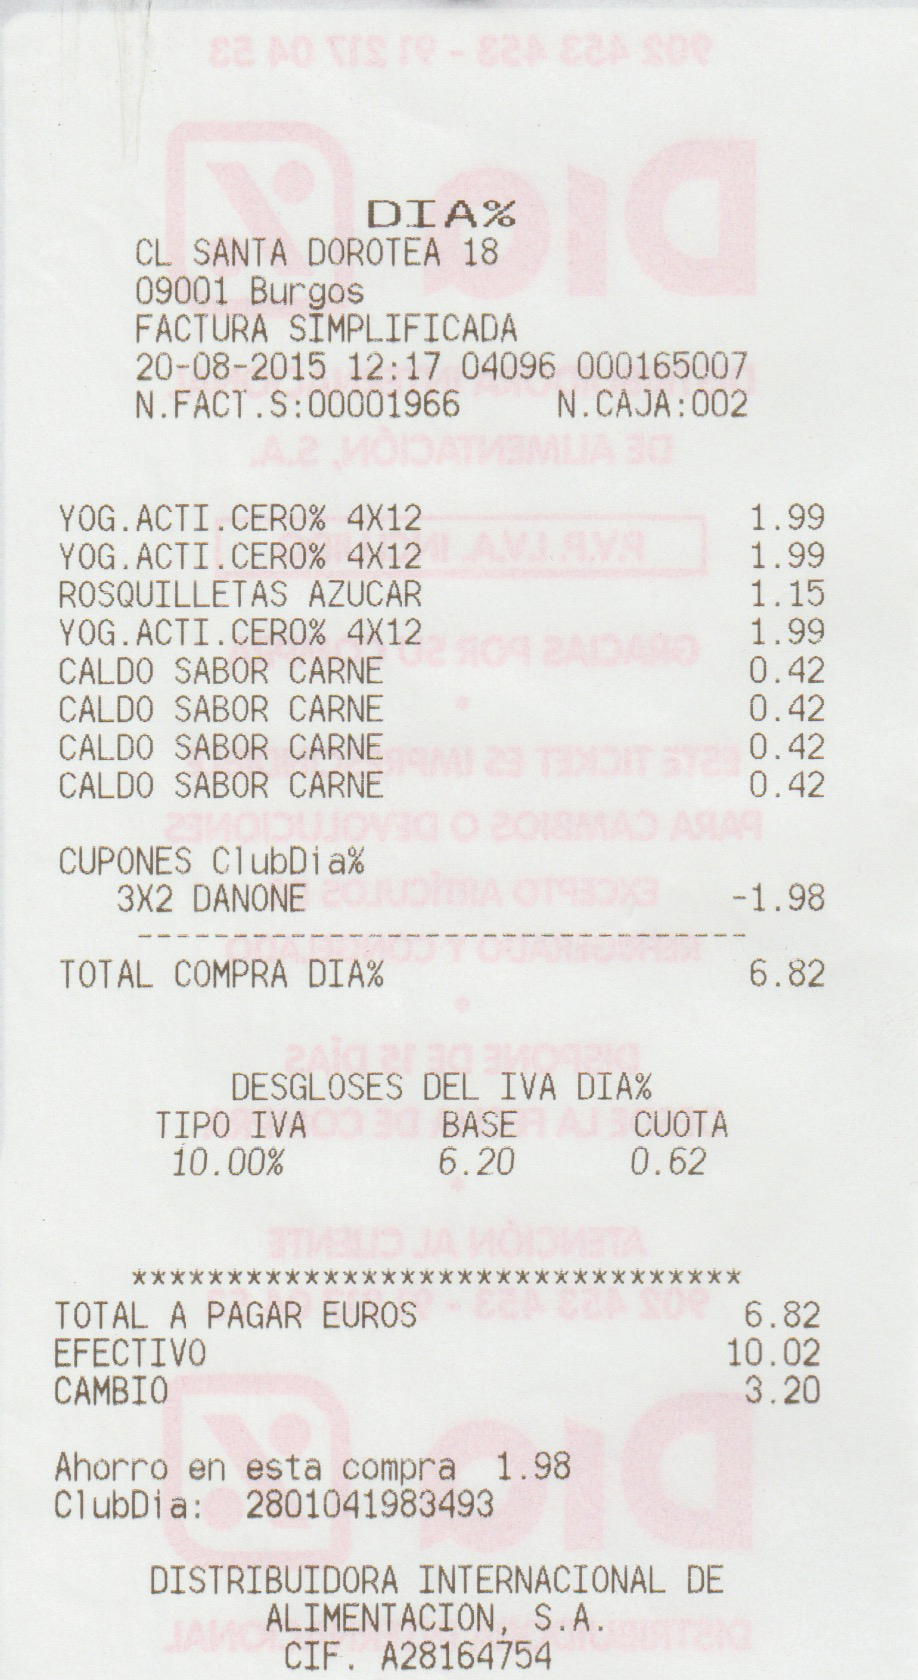
\includegraphics[width=\linewidth]{tique1.jpg}
			\caption{Tique con 2 columnas}
			\label{fig:minipage1}
	\end{minipage}
	\quad
	\begin{minipage}[b]{0.45\linewidth}
		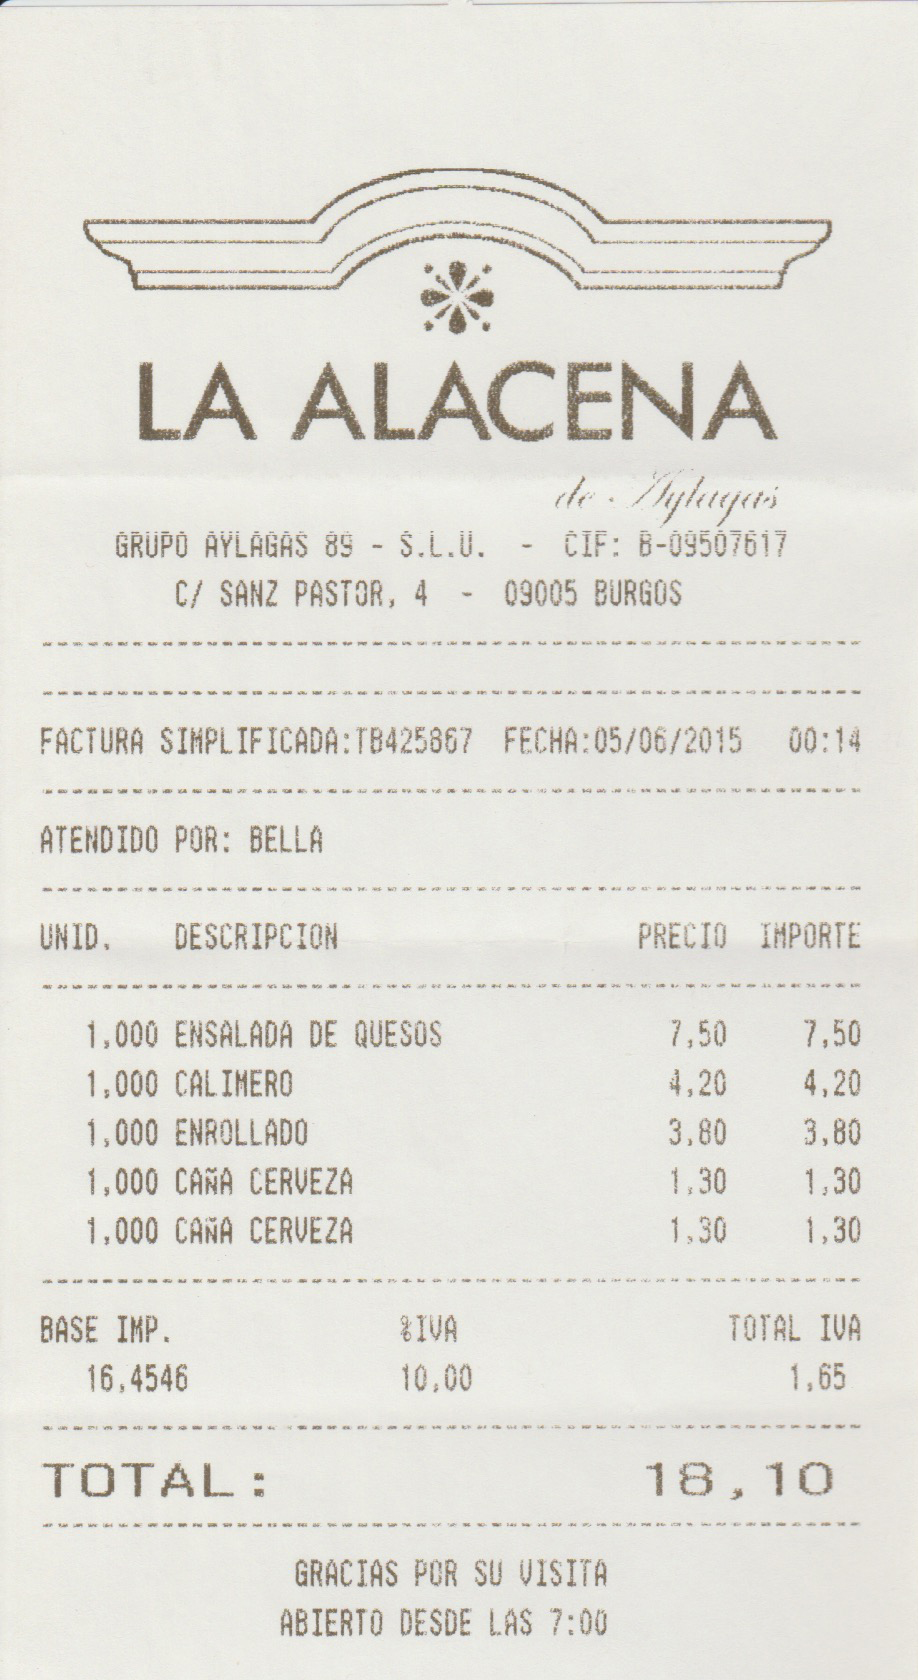
\includegraphics[width=\linewidth]{tique2.jpg}
		\caption{Tique con 4 columnas}
		\label{fig:minipage2}
		\end{minipage}
		\quad
		\begin{minipage}[b]{0.45\linewidth}
			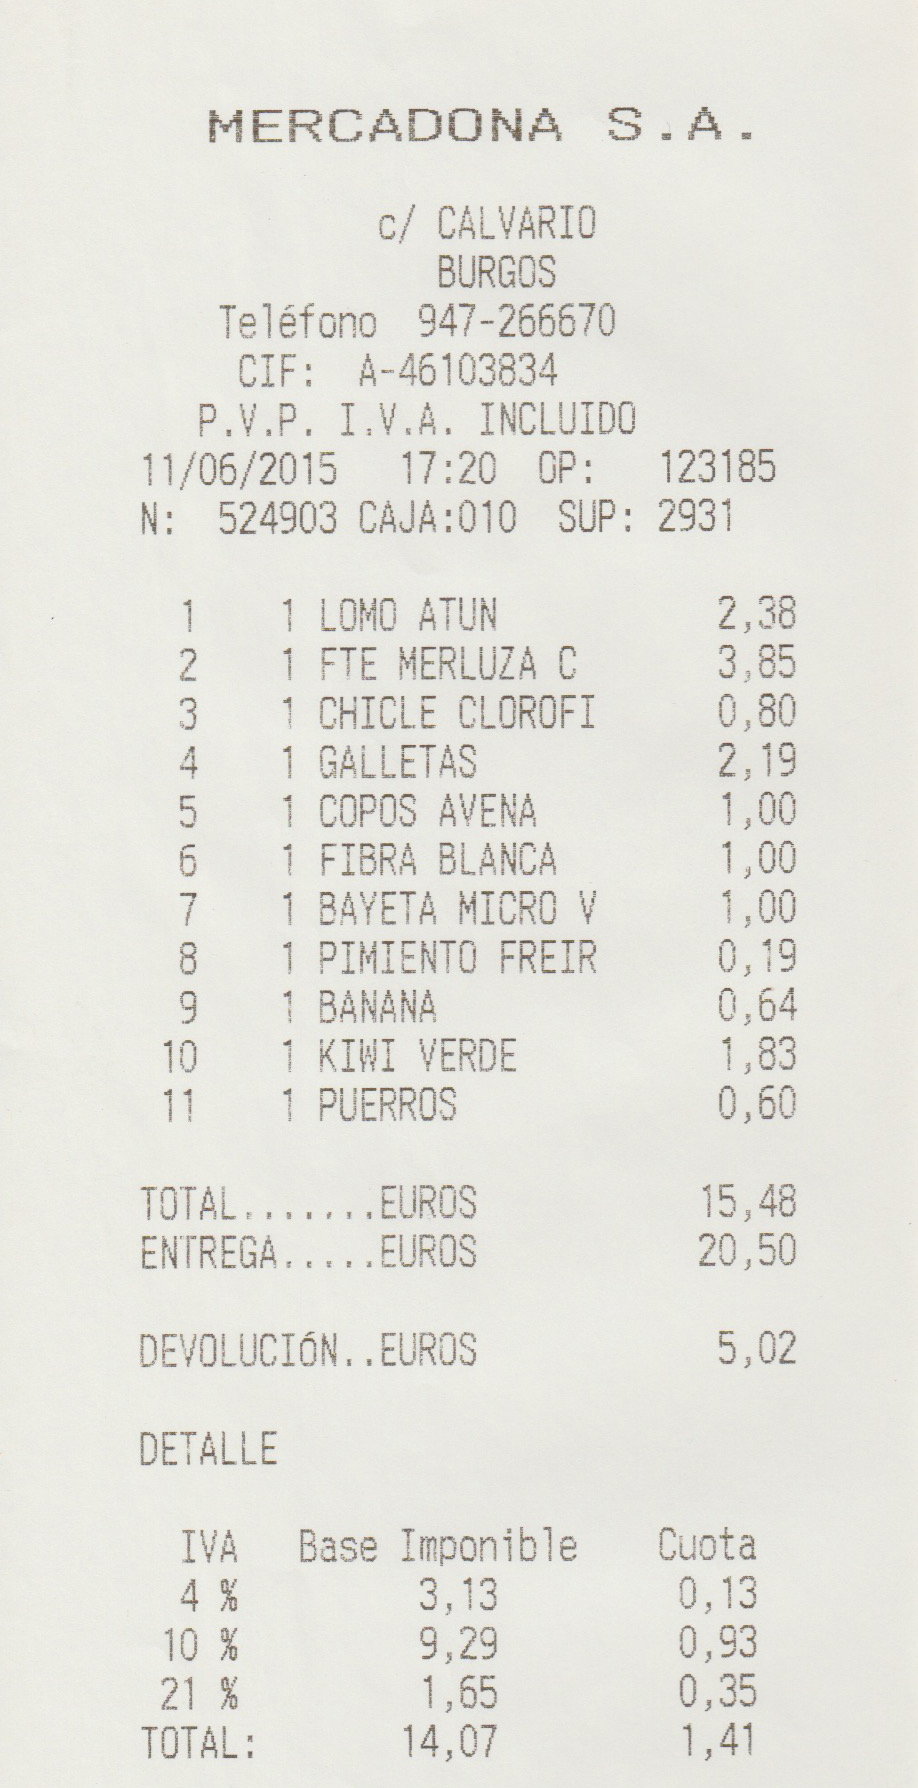
\includegraphics[width=\linewidth]{tique3.jpg}
			\caption{Tique con 4 columnas}
			\label{fig:minipage3}
	\end{minipage}
	\quad
	\begin{minipage}[b]{0.45\linewidth}
		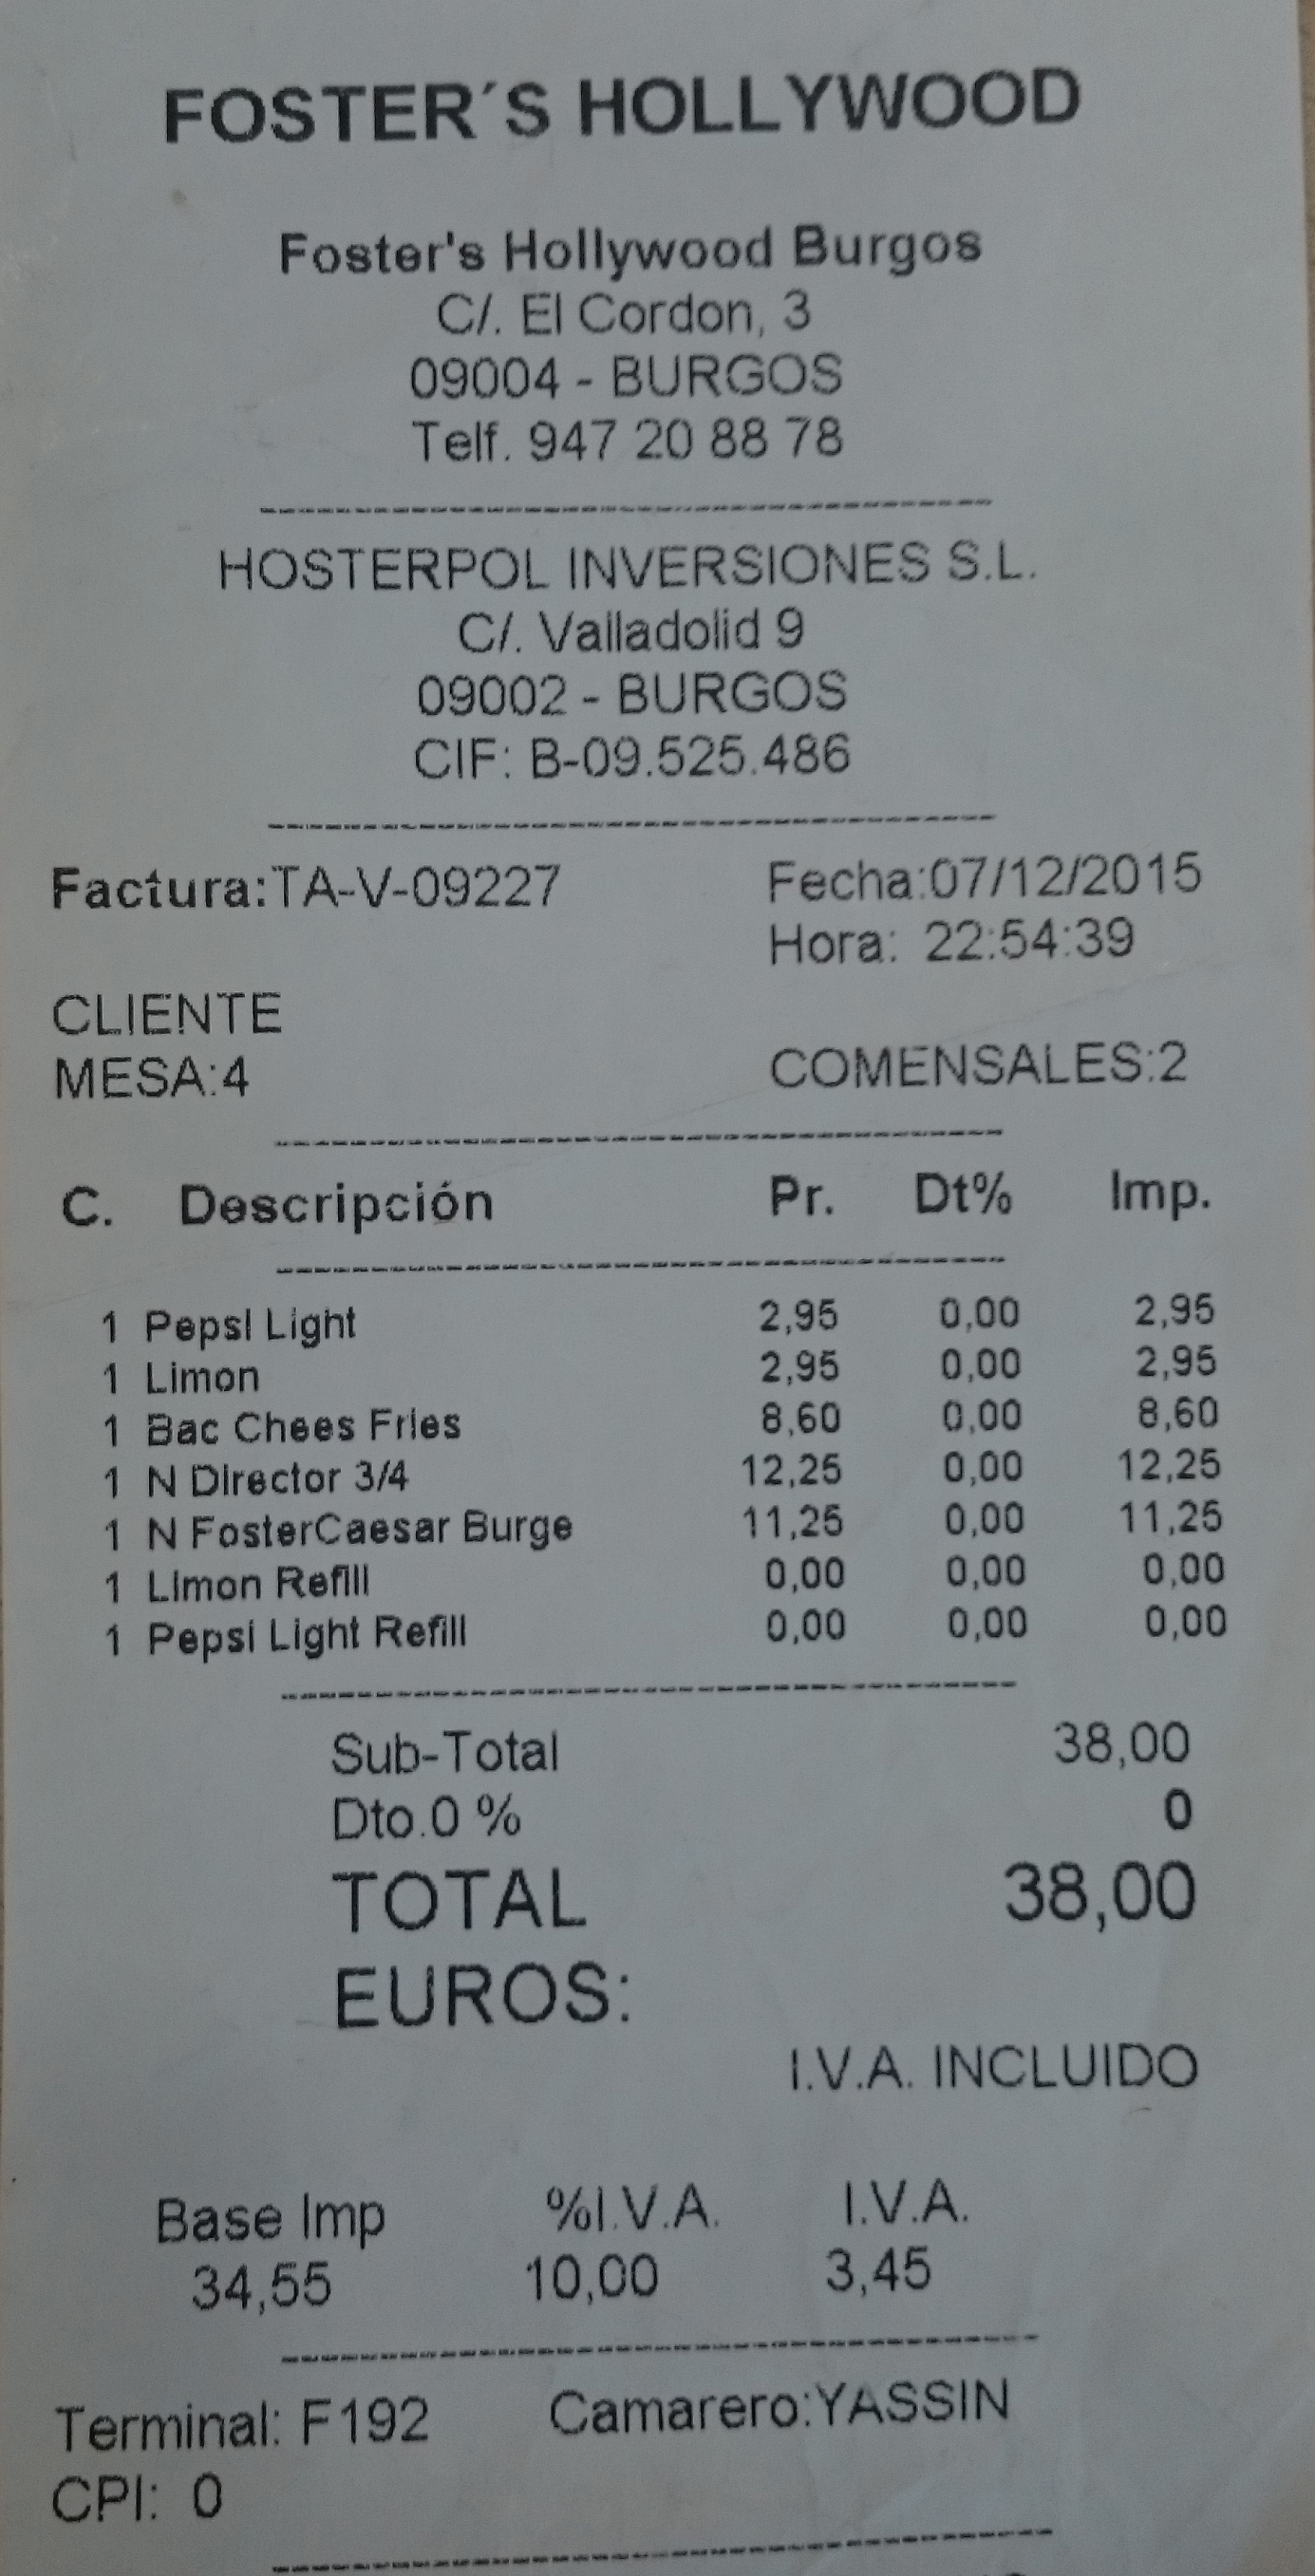
\includegraphics[width=\linewidth]{tique4.jpg}
		\caption{Tique con 5 columnas}
		\label{fig:minipage4}
		\end{minipage}
\end{figure}

\cleardoublepage

Podemos ver como en cada tique las columnas en las que se distribuye la información varía de uno a otro, sin embargo, en los muchos tiques que siguen una distribución de 4 columnas (ver figura \ref{fig:minipage2}) estas se distribuyen de la siguiente manera:
\begin{itemize}
	\item Unidades.
	\item Descripción.
	\item Precio.
	\item Importe.
\end{itemize}

Por lo que es posible abarcar un numero elevado de tiques, ya que este modelo, se emplea principalmente en establecimientos de hostelería y restauración.


\section{Modelo Cliente-Servidor}

La arquitectura cliente-servidor es un modelo de aplicación distribuida en cual las que las tareas se reparten entre los proveedores de servicios o servidores, y los demandantes denominados clientes \cite{wiki:Cliente-servidor}.

El cliente realiza las peticiones a un programa, que se encuentra en el servidor, y este le devuelve una respuesta de vuelta al cliente (ver figura \ref{fig:client_server}), por ello toda la gestión de la información y responsabilidad se encuentra en el servidor.

\imagen{client_server}{Peticion-Respuesta de un cliente a un servidor}

Las ventajas de este tipo de arquitectura son: 
\begin{itemize}
	\item \textbf{Uso de recursos:} El uso de un servidor permite a los clientes el uso de los recursos de este, lo que facilita la ejecución de tareas mas costosas en un tiempo menor.
	\item \textbf{Escalabilidad:} Es posible añadir nuevos clientes en cualquier momento.
	\item \textbf{Facilidad de mantenimiento:} Dado que el cliente y el servidor son maquinas distintas, es posible realizar cambios en este ultimo sin que el cliente se vea afectado, lo que permite añadir nuevas funcionalidades sin la necesidad de cambiar los clientes.
\end{itemize}

Sin embargo, este modelo presenta dos desventajas muy claras:
\begin{itemize}
	\item \textbf{Necesidad de una conexión:} Es necesario mantener un canal de conexión entre el cliente y el servidor.
	\item \textbf{Disponibilidad:} El servidor debe estar disponible en todo momento, dado que el resto de maquinas depende de el.
\end{itemize}

La mayoría de los servicios que se proporcionan en la actualizad utilizan esta estructura.


\section{Api-Rest}
Representational State Transfer o Rest es una arquitectura software apoyada en un modelo cliente-servidor y el protocolo HTTP \cite{wiki:rest}.

Este modelo se utiliza para definir a un sistema que utiliza el protocolo HTTP para realizar llamadas al servidor con una serie de parámetros, los cuales son los datos  a interpretar por el servidor, una vez procesados se genera una respuesta que se devuelve al cliente, generalmente en formato XML o JSON.

En el presente trabajo, se ha construido un servicio REST que recibe como parámetro una imagen de un tique y devolver los productos que se han encontrado en este, empaquetados en un JSON.

\section{JSON}

JSON es un acronimo para JavaScript Objet Notation, es un estandar de texto plano, empleado para el intercambio de datos. La ventaja de este formato es que es independiente del lenguaje de programación en los que las maquinas están programadas, cada lenguaje tiene su propia librería para codificar y descodificar cadenas JSON \cite{json}.

La formación de un objeto JSON se realiza con pares atributo-valor que deben estar encerrados entre llaves y separados por comas, las cuales definen el principio y el fin del objeto.

Un ejemplo: \textit{$\{
"nombre":"Roberto",
"edad":23
\}$}
